\documentclass[fleqn]{article}

\usepackage{listings}
\usepackage[german]{babel}
\usepackage[T1]{fontenc}
\usepackage[latin1]{inputenc}
\usepackage{titlesec}
\usepackage{geometry}
\usepackage{qtree}
\usepackage{tikz}
\usepackage{amsmath}
\setcounter{secnumdepth}{0}
\usetikzlibrary{positioning}
\geometry{top=2.5cm, bottom=2.5cm}
\lstset{
 columns=fixed,       
 numbers=left,                                        % 在左侧显示行号
 numberstyle=\tiny\color{gray},                       % 设定行号格式
 frame=none,                                          % 不显示背景边框
 backgroundcolor=\color[RGB]{245,245,244},            % 设定背景颜色
 keywordstyle=\color[RGB]{40,40,255},                 % 设定关键字颜色
 numberstyle=\footnotesize\color{darkgray},           
 commentstyle=\it\color[RGB]{0,96,96},                % 设置代码注释的格式
 stringstyle=\rmfamily\slshape\color[RGB]{128,0,0},   % 设置字符串格式
 showstringspaces=false,                              % 不显示字符串中的空格
 language=sql,                                        % 设置语言
 breaklines,                                          % 自动换行
}
\begin{document}

\newpagestyle{main}{
    \sethead{Matrikel-Nr.: 574145 Dongze Yang}{}{}
    \setfoot{}{\thepage}{}
    \headrule
    \footrule
}
\pagestyle{main}
%\section{Aufgabe}

\section{1. Aufgabe}

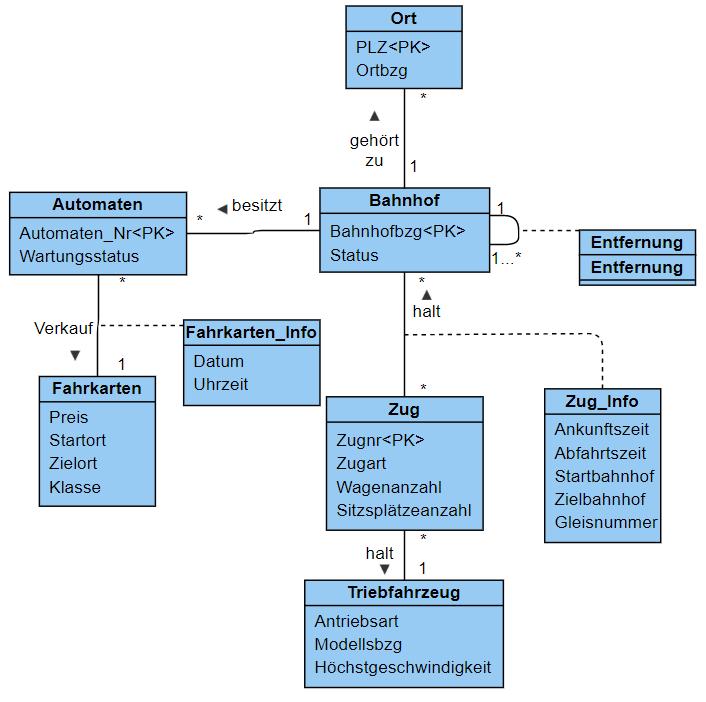
\includegraphics[scale=0.6]{UML.png}

\section{2. Aufgabe}

Wohnung(\underline{Wohnungsnr}, Straße, Hausnummer, Postleitzahl, Stadt, Land)\\
Mietinfomationen(\underline{MietInfoNr}, Wohnungsnr, Einzugsdatum, Kaltmiete)\\
Person(\underline{PersonsNr}, Wohnungsnr, Name, Vorname, Geschleicht, Hobby, Eltern, Kind)\\

\section{3. Aufgabe}

Daten umschreiben
\begin{lstlisting}
    INSERT INTO gesell (gesell_bez, hauptsitz, land)
    VALUES ('EASYJET', 'UK', 'Luton')
    UPDATE bestand
    SET gesell_bez = 'EASYJET'
    WHERE gesell_bez = 'AIR BERLIN'
    UPDATE angestellt
    SET gesell_bez = 'EASYJET'
    WHERE gesell_bez = 'AIR BERLIN'
    DELETE gesellWHERE gesell_bez = 'AIR BERLIN'
\end{lstlisting}
Flugzeugflotte
\begin{lstlisting}
    SELECT M.fznr, F.sitze, F.geschw
    FROM maschine M, fztyp F
    WHERE M.typ = F.typ
\end{lstlisting}
Piloten
\begin{lstlisting}
    SELECT P.pinr
    FROM P.pinr, Count(F.fnr)
    FROM flug F, pilot P
    WHERE F.pinr = P.pinr
        AND F.datum > '01-01-2000'
\end{lstlisting}

\section{4. Aufgabe}

(a)
\begin{lstlisting}
    SELECT gehalt
    FROM personal
    ORDER BY ASC
\end{lstlisting}
(b)
\begin{lstlisting}
    SELECT pnr, ort
    FROM personal
         NATURAL JOIN abteilung
    ORDER BY ort
\end{lstlisting}
(c)
\begin{lstlisting}
    SELECT Pers.name, Pers.Vorname, Pro.Name
    FROM personal Pers, projekt Pro
    WHERE Pers.PNr IN (SELECT leiter FROM Pro)
\end{lstlisting}
(d)
\begin{lstlisting}
    SELECT Sum(Pers.gehalt)
    FROM personal PersWHERE Pers.PNr IN (
        SELECT DISTINCT (Z.PeNr)
        FROM zuordnung Z
        WHERE P.PrNr IN (
            SELECT P.PNrFROM projekt P
            WHERE P.leiter = 50
        )
    )
\end{lstlisting}
(e)
\begin{lstlisting}
    SELECT Avg (P.gehalt)
    FROM personal P
    WHERE P.PNr IN(
        SELECT Z.PeNr
        FROM zuordnung Z
        GROUP BY Z.PrNr
    )
\end{lstlisting}
(f)
\begin{lstlisting}
    SELECT Pro.name
    FROM projekt Pro
    WHERE Pro.PNr IN(
        SELECT Z.PrNr
        FROM zuordnung Z
        WHERE Z.PeNr IN (
            SELECT P.PNr
            FROM personal P
            WHERE P.gehalt >=1000
        )
    )
\end{lstlisting}
(g)
\begin{lstlisting}
    SELECT Pro.name, P.name, P.vorname
    FROM projekt Pro, personal P, zuordnung Z
    WHERE Z.PeNr = P.PNr
    ORDER BY Pro.budget DESC, P.name ASC, P.vorname ASC
\end{lstlisting}

\section{5. Aufgabe}

(a)
Startflughafen$ \_ $ID $\rightarrow$ Startort

Landeflughafen$ \_ $ID $\rightarrow$ Landeort

(Startflughafen$ \_ $ID, Landeflughafen$ \_ $ID) $\rightarrow$ Entfernung

(Startzeit, Startflughafen$ \_ $ID, Landeflughafen$ \_ $ID) $\rightarrow$ Landezeit

Schlüsselkandidat: (Flugnr, Flugabschnittnr)
\\
(b)
Die Relation befindet sich in 1NF und 2NF.
\\
(c)

Einfüge-Anomalie: Wenn derselbe Flug an verschiedenen Tagen durchgeführt wird, muss jeder Abflug- und Landeflughafen erfasst werden.

Lösch-Anomalie: Fluginformationen werden gelöscht, wenn die Flugabschnitt gelöscht werden.

Update-Anomalie: 
\\
(d)

Flughafen( \underline{Flughafen\_ID}, Ort)

\end{document}